\documentclass[./main.tex]{subfiles}

\begin{document}
\section{Analisi esplorativa}
Per condurre una prima analisi esplorativa le tecniche d'analisi utilizzate sono state le seguenti:
\begin{itemize}
	\item PCA sui dati sbiancati.
	\item ICA sui dati sbiancati.
	\item t-SNE.
	\item t-SNE sui dati sbiancati.
\end{itemize}
I risultati ottenuti:
\begin{figure}[H]
	\centering
	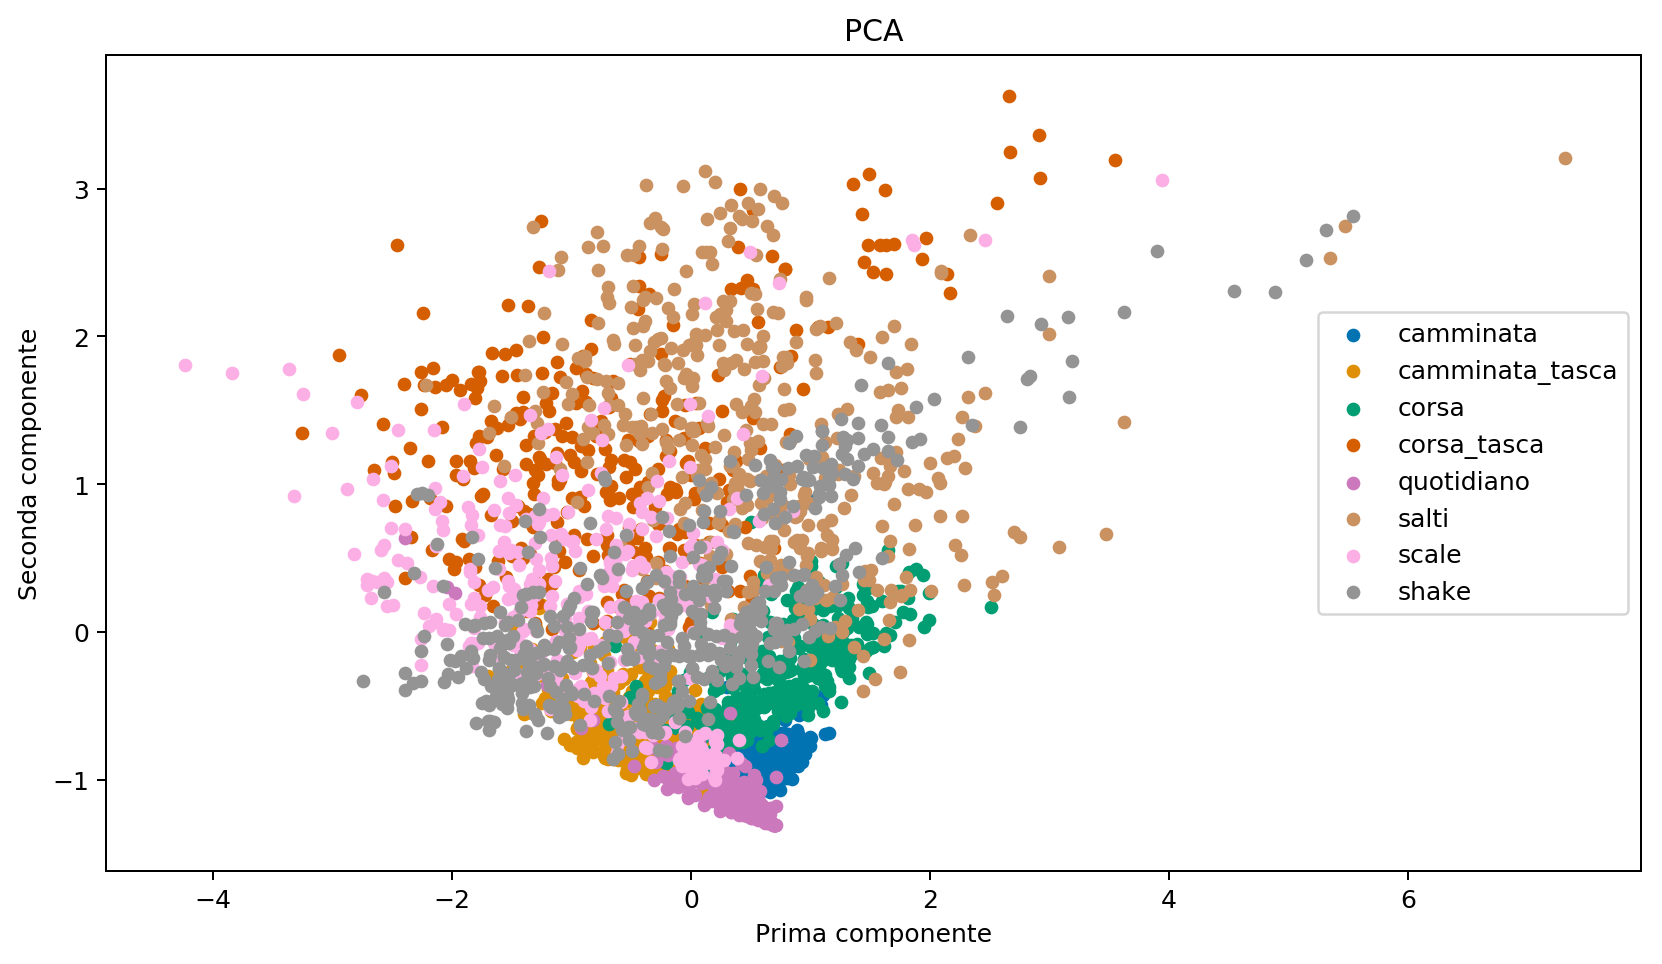
\includegraphics[width=.99\textwidth, keepaspectratio]{../../figure/PCA.png}
	\caption{{ Prime due componenti principali per i dati sbiancati}}
	\label{PCA}
\end{figure}

%\begin{figure}[H]
%	\centering
%	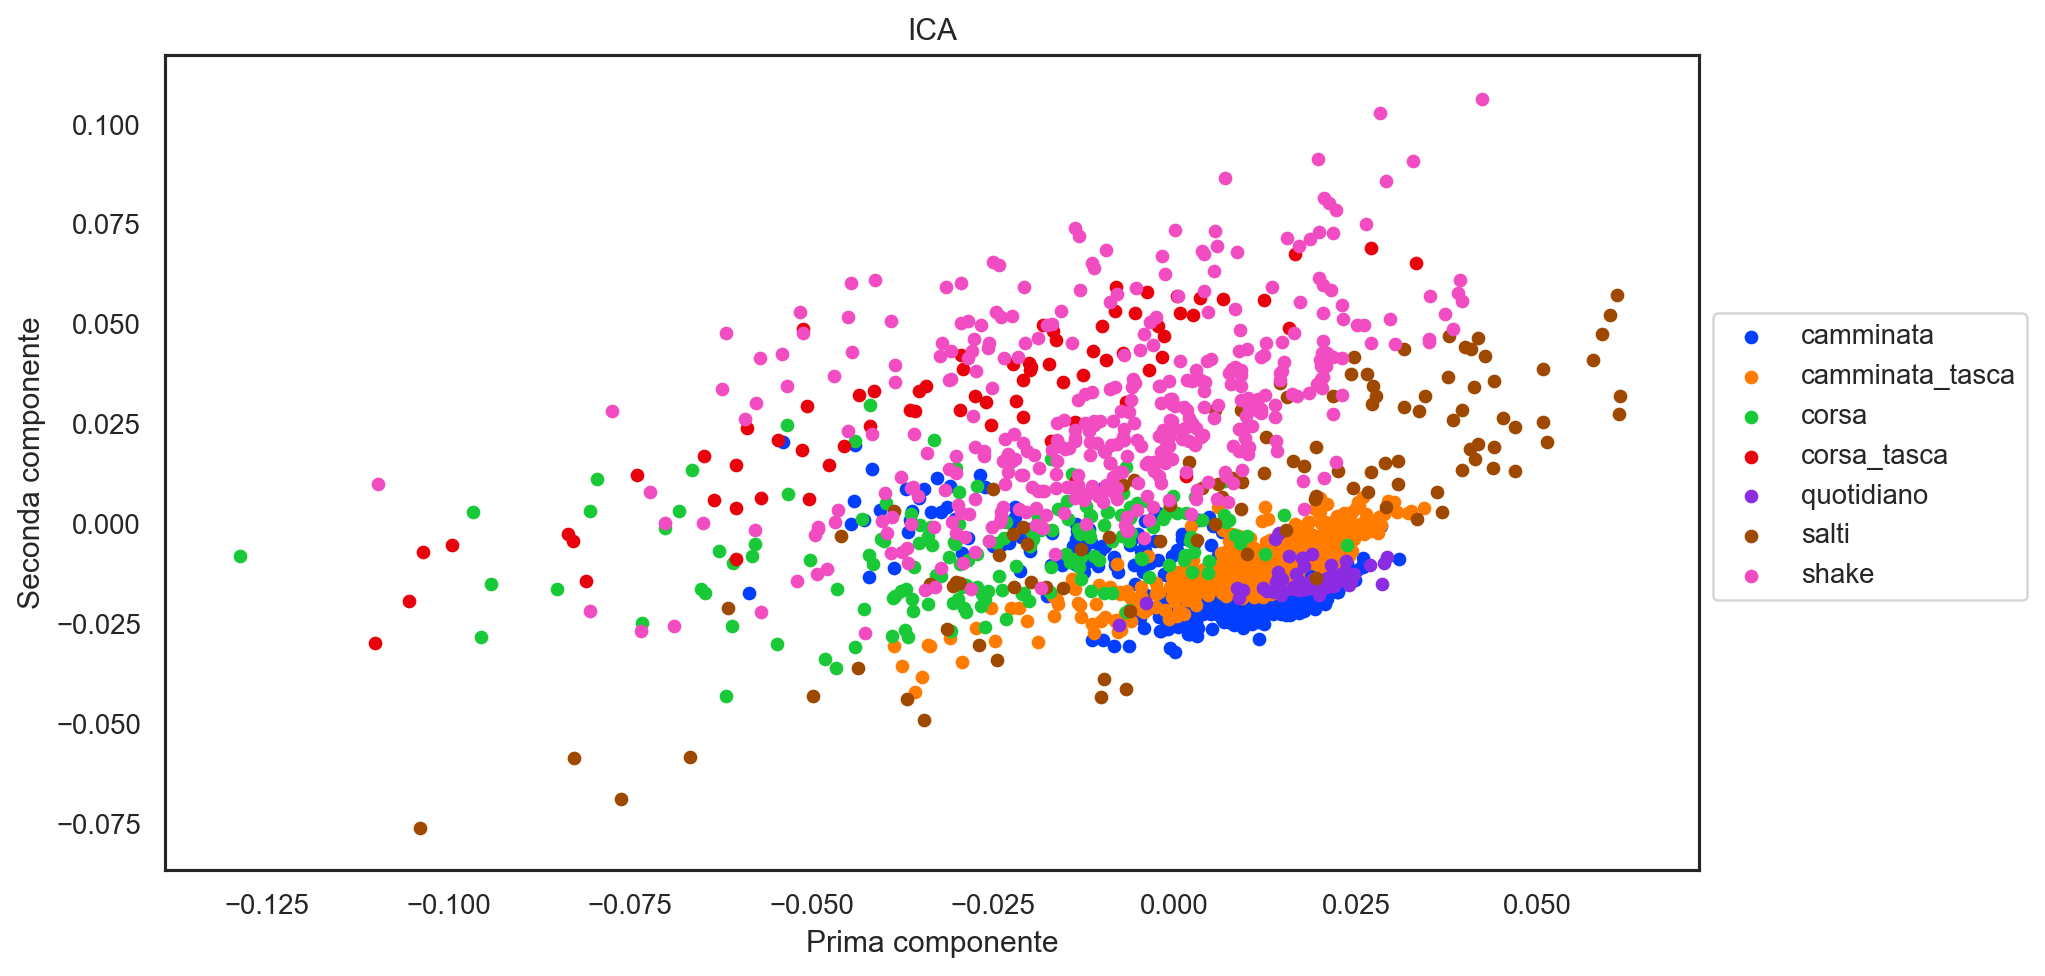
\includegraphics[width=.99\textwidth, keepaspectratio]{../../figure/ICA.png}
%	\caption{{ Analisi esplorativa con ICA su dati sbiancati}}
%	\label{ICA}
%\end{figure}

\begin{figure}[H]
	\centering
	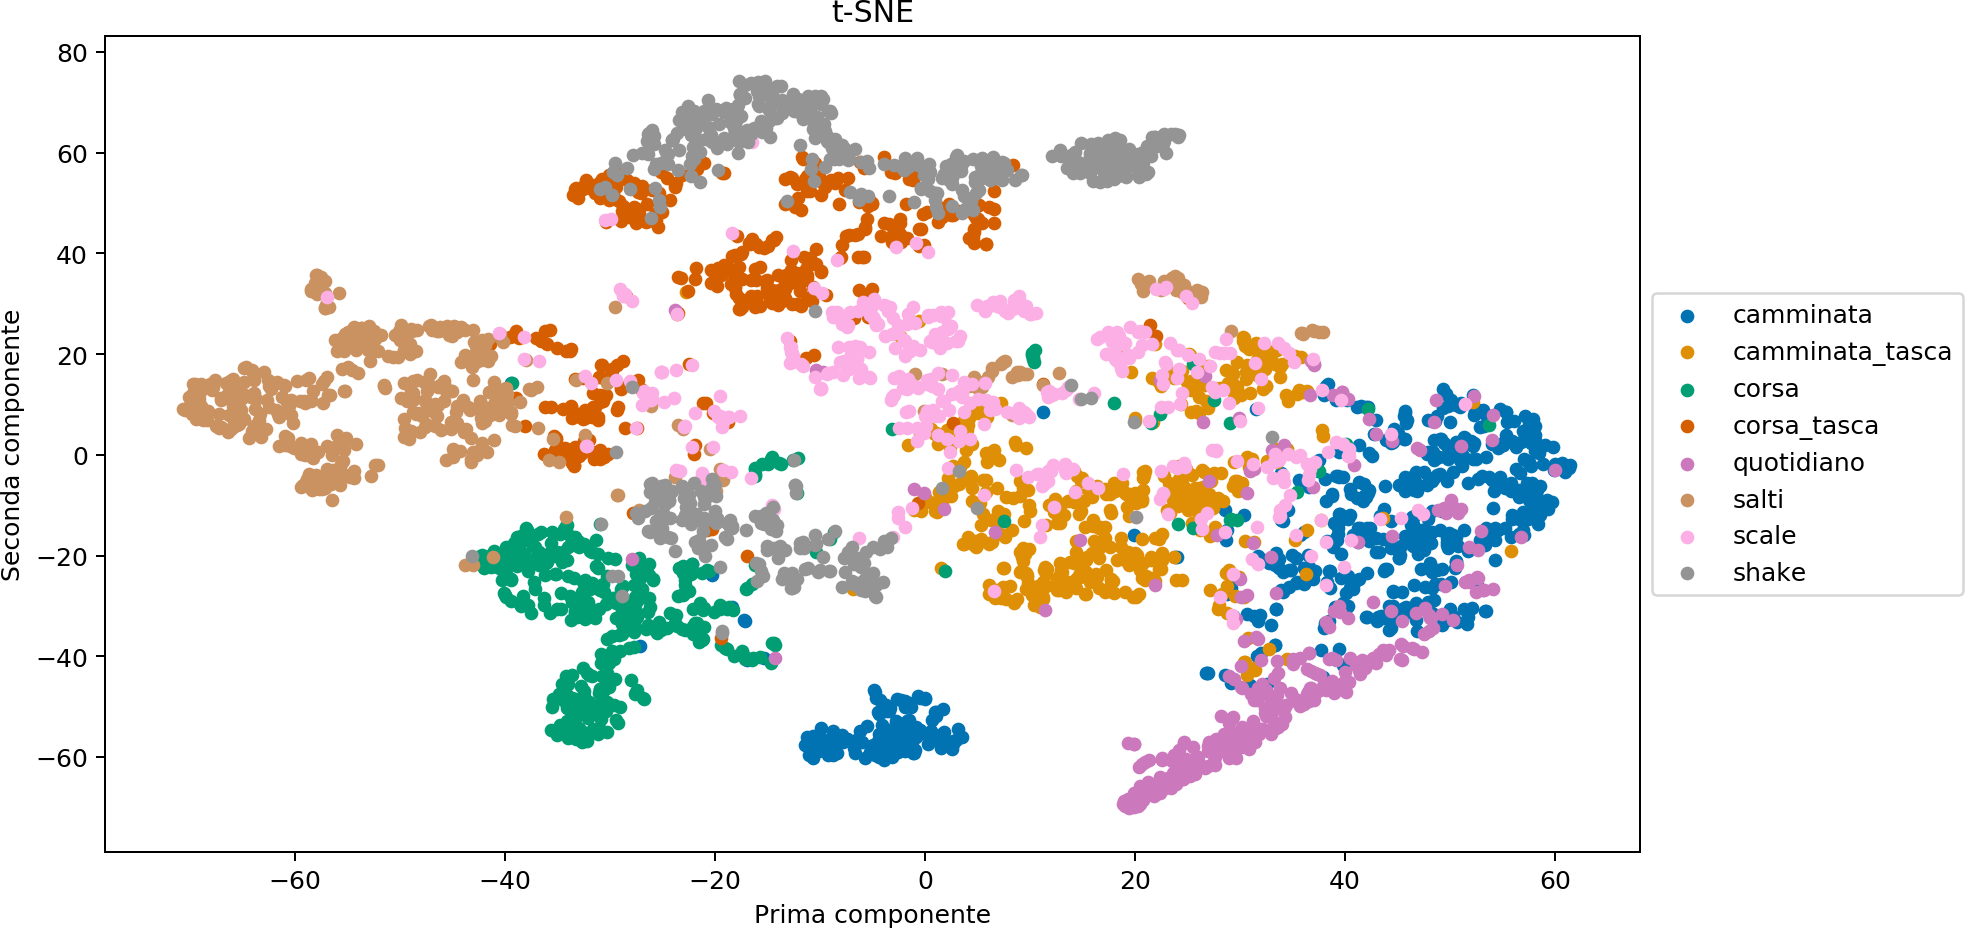
\includegraphics[width=.99\textwidth, keepaspectratio]{../../figure/t-SNE.png}
	\caption{{ t-SNE per i dati sbiancati}}
	\label{tSNE}
\end{figure}
Al fine di riuscire a discriminare l'azione svolta, classificata in "camminata", "camminata tasca", "corsa", "corsa tasca", "quotidiano", e "shake", sono stati applicati i seguenti algoritmi di classificazione:
\begin{itemize}
	\item Regressione multinomiale.
	\item Alberi di classificazione.
\end{itemize}


\end{document}